\documentclass{beamer}

\usepackage[utf8]{inputenc}
\graphicspath{{../Graphics/}}

%Information to be included in the title page:
\title{Heat Energy Sources in Canada}
\author{Noah Bolohan, Anton Iatcenko, Ryan Thiessen, Yakine Bahri, Benjamin MacAdam, Alireza Yazdani}
\institute{Math\textsuperscript{Industry}}

\date{August 2020  \\ \vspace{30pt} 
\includegraphics[scale=0.3]{pims_logo.png} }



\begin{document}

\frame{\titlepage}

\begin{frame}
\frametitle{The Data Set (Yakine)}
what the data is, where it came from
\end{frame}


\begin{frame}
\frametitle{The Big Picture (Noah)}
Canada as a whole (pie chart)
\end{frame}


\begin{frame}
\frametitle{Change Over Time I (Anton)}
stacked bars (4 per slide)
\end{frame}


\begin{frame}
\frametitle{Change Over Time II (Anton)}
stacked bars (4 per slide)
\end{frame}


\begin{frame}
\frametitle{Change Over Time III (Anton)}
stacked bars (4 per slide)
\end{frame}


\begin{frame}
\frametitle{Province Groupings (Anton)}
stacked bars (all together)
\end{frame}


\begin{frame}
\frametitle{Cause of the Groupings: Natural Gas (Ryan)}

\end{frame}


\begin{frame}
\frametitle{Cause of the Groupings: Electricity (Alireza)}

\end{frame}


\begin{frame}
\frametitle{Cause of the Groupings: Atlantic Provinces (Ben)}
	
	\begin{tabular}{ c c}
	  \scalebox{0.3}{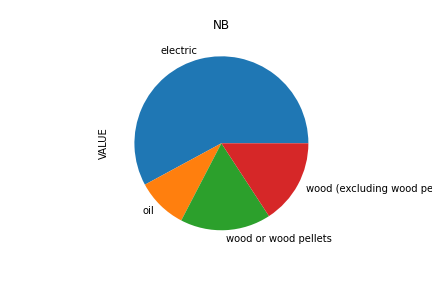
\includegraphics{Ben_Images/NB.png}}
	& \scalebox{0.3}{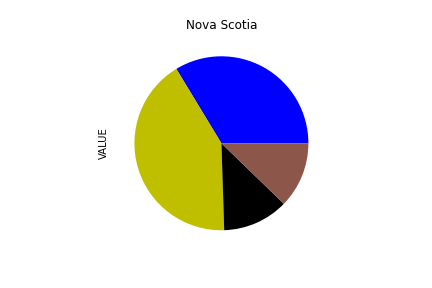
\includegraphics{Ben_Images/NS.png}} \\
	\scalebox{0.3}{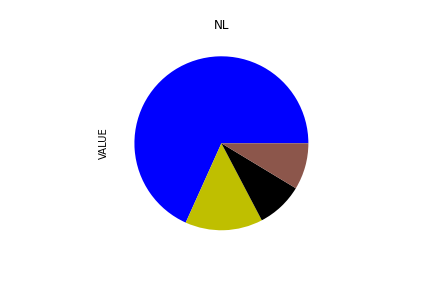
\includegraphics{Ben_Images/NL.png}}
	& \scalebox{0.3}{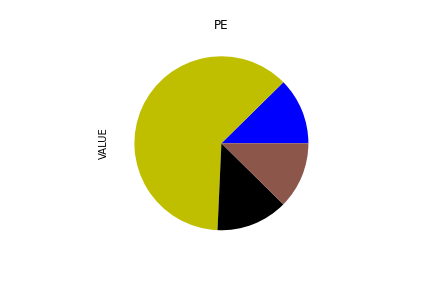
\includegraphics{Ben_Images/PE.png}}
	\end{tabular}
	Same story in Atlantic region:
	\begin{itemize}
		\item Newfoundland,New Brunswick: Access to hydro, use electric.
		\item Prince Edward Island, Nova Scotia: No hydro access, use oil.
	\end{itemize}
\end{frame}


\begin{frame}
\frametitle{Summary}

No change over time. 

The dependence is predominantly geographic. 

Thanks for your attention.  

\end{frame}













\end{document}



















